\documentclass[border=2pt]{standalone}
\usepackage{tikz}
\usetikzlibrary{arrows.meta,topaths}

\begin{document}
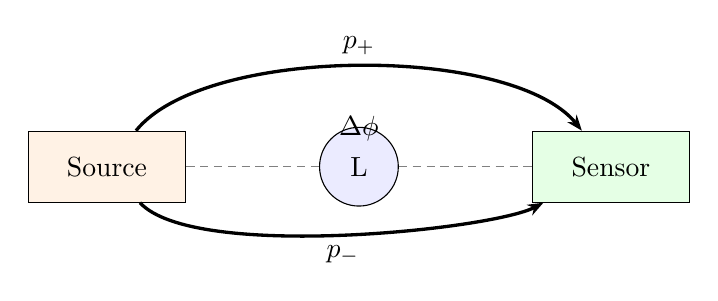
\begin{tikzpicture}[
  device/.style={draw,minimum width=20mm,minimum height=9mm,align=center},
  ray/.style={-{Stealth[length=2mm]},very thick}
]
  \node[device,fill=orange!10] (source) at (0,0) {Source};
  \node[draw,circle,minimum size=10mm,fill=blue!8] (lens) at (3.2,0) {L};
  \node[device,fill=green!10] (sensor) at (6.4,0) {Sensor};

  \path[ray]
    (source) edge[controls={+(1.25,1.55) and +(-1.25,1.55)}] node[above] {$p_+$} (sensor)
    (source) edge[out control={+(1.1,-1.2)},in control={+(-1.5,-0.8)}] node[below] {$p_-$} (sensor);
  \draw[densely dashed,gray] (source) -- (lens) -- (sensor);
  \node[above=2mm] at (lens) {$\Delta\phi$};
\end{tikzpicture}
\end{document}
